%% Hello emacs, this is -*- latex -*-
\typeout{ ====================================================================}
\typeout{ This is file coord-atlas.tex, created at 24-Feb-2004 }
\typeout{ Maintained by Andre DOS ANJOS <Andre.dos.Anjos@cern.ch> }
\typeout{ ====================================================================}

\chapter{As Coordenadas do ATLAS}
\label{ap:coord}
\index{ATLAS!coordenadas}

O sistema de coordenadas usado em experimentos com feixes não é, em muitos
casos, o sistema polar. É um sistema adequado ao formato cilíndrico dos
detetores dispostos ao redor do ponto de impacto, ou seja, um sistema que
\emph{acompanha} a direção dos feixes de partículas provenientes da
colisão. As coordenadas empregadas são $\eta$, $\phi$ e \textit{z} em
contraposição a \textit{x}, \textit{y} e \textit{z}. $\eta$ e $phi$ seguem a
uma transformação não-linear de \textit{x} e \textit{y}:

\begin{equation}
\phi = \text{atan}({\frac{x}{y}})
\end{equation}
\begin{equation}
\eta = - \log({\tan({\frac{\phi}{2}})})
\end{equation}

A figura~\ref{fig:etaphi} pode ser explicativa quanto ao sistema. Em sua parte
superior, é possível ver um esquema do barril e da tampa de um detetor,
mostrando como se comportam as coordenadas tomando por referência as
coordenadas cartesianas \textit{x}, \textit{y} e \textit{z} (marcadas em
pontilhado). Nota-se que a variável $\phi$ representa a rotação e a variável
$\eta$ (também chamada de pseudo-rapidez\index{pseudo-rapidez}) representa a
direção de projeção das partículas, após a colisão.

Os valores dados das variáveis $\eta$ e $\phi$ são apenas para referência do
leitor. A variável $\phi$, como é possível ver no canto direito da parte
superior da figura, possui uma região em que dois valores são possíveis: 0 e
2$\pi$. Esta área é chamada de região \eng{wrap-around}. Cálculos utilizando
esta variável devem atentar para este fato. Os detetores são simétricos, com
relação ao eixo $\phi$. A construção dos dispositivos é feita em gomos.

Nota-se que quando alcança o eixo \textit{z}, $\eta = \infty$, isto significa
que objetos com valores grandes em $\eta$ representam colisões onde as
partículas do feixe apenas se desviaram, não havendo, usualmente, informações
interessantes de análise, pois representam choques elásticos. É comum
utilizarem-se detetores com baixa resolução quando $eta > 3$.

\begin{figure}
\begin{center}
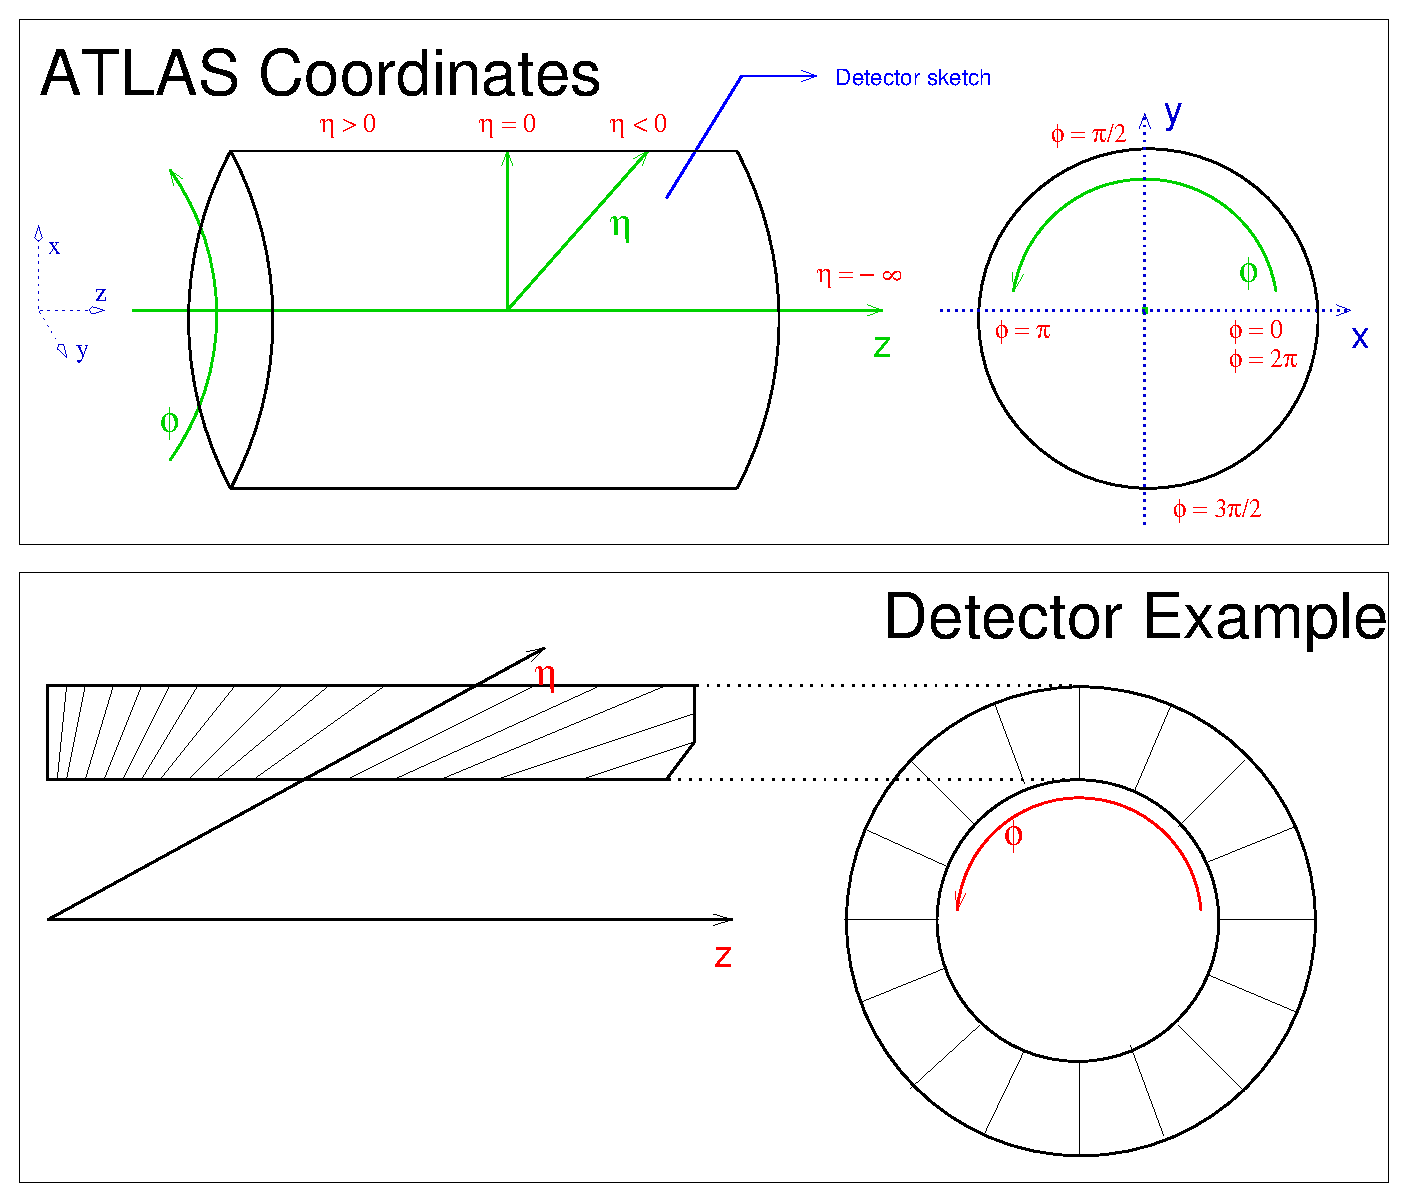
\includegraphics[scale=0.6]{etaphi}
\end{center}
\caption{O sistema de coordenadas do ATLAS.}
\label{fig:etaphi}
\end{figure}

Na parte inferior da figura~\ref{fig:etaphi}, é possível ver um exemplo de
como um detetor genérico é segmentado, acompanhando as coordenadas $eta$ e
$\phi$, tanto para o barril, quanto para uma tampa.

\typeout{ *************** End of file coord-atlas.tex *************** }
